\documentclass[12pt]{article}

\usepackage{amsfonts}
\usepackage{amsthm}
\usepackage{amsmath}
\usepackage{amssymb}
\usepackage{makecell}
\usepackage{mathtools}
\usepackage{dsfont}
\usepackage{xcolor}
\usepackage[normalem]{ulem}
\usepackage{hyperref}
\hypersetup{
    colorlinks=true,
    linkcolor=blue
}
\usepackage{algorithm}% http://ctan.org/pkg/algorithm
\usepackage{algpseudocode}% http://ctan.org/pkg/algorithmicx



\newcommand{\floor}[1]{\lfloor #1 \rfloor}
\newcommand{\FF}{\mathbb{F}}
\newcommand{\ZZ}{\mathbb{Z}}
\newcommand{\LL}{\mathcal{L}}
\DeclareMathOperator{\Span}{Span}


\newtheorem{question}{Question}
\newtheorem{lemma}{Lemma}
\newtheorem{theorem}{Theorem}
\newtheorem{remark}{Remark}
\newtheorem{definition}{Definition}
\newtheorem{corrolary}{Corrolary}



\title{Comparing Lattice Families for Bounded Distance Decoding near Minkowski’s Bound}

\author{ Oleksandra Lapiha }
\usepackage{xcolor}
\def\added{\bgroup \markoverwith{\textcolor{green!50!blue}{\lower4.5pt\hbox{\sixly \char58}}}\ULon}
\def\toimprove{\bgroup \markoverwith{\textcolor{red}{\lower4.5pt\hbox{\sixly \char58}}}\ULon}
\def\improved{\bgroup \markoverwith{\textcolor{black}{\lower4.5pt\hbox{\sixly \char58}}}\ULon}


\begin{document}

\maketitle



\section{Introduction}
\label{sec:intro}



\textbf{Bounded Distance Decoding problem.}

Message decoding is a problem that arises when two parties need to communicate over a noisy channel. Here we are in the setting where we are only concerned with the integrity of transmitted data and we assume there's no adversary listening and modifying messages in the network. We are dealing with information loss that occurs due to our information flow being \textit{slightly disturbed} by forces of nature.

To achieve that we encode messages as points in Euclidean space. Now we can model the rate of "disturbance" as distance between the input and output points. And call it "slight" if it can be bounded by a constant. A natural way to arrange the space of messages is a Euclidean lattice(all integer linear combinations of a linearly independent set of vectors in $\mathbb{R}^{n}$).

The decoding procedure aims to identify the point of the lattice closest to the output point. If the disturbance in the network is small enough the closest lattice point will indeed be the input message. This will help us identify the upper bound on how much error a perfect decoding algorithm can handle. We know that the distance between lattice points is bounded from below by the length of the shortest vector($\lambda_{1}(\LL)$) of the lattice. If the error exceeds $\frac{\lambda_{1}(\LL)}{2}$, the closest point might not be the input message anymore so decoding becomes impossible.

We would like to have an algorithm where the decoding radius is close to $\frac{\lambda_{1}(\LL)}{2}$. Unfortunately, the Lattice Shortest Vector Problem(SVP) is believed to be hard in the general case, so we cannot evaluate exactly how good our decoding radius is. Nevertheless, we have an upper-bound on the length of the shortest vector. So we aim to get a decoding radius close to it instead.
\begin{theorem}[Minkowski's First Theorem]
    For any full-rank lattice $\LL$ of rank $n$,
    \[
        \lambda_{1}(\LL) \leq \sqrt{n} \det(\LL)^{1/n}
    \]
\end{theorem}

An instance of such problem is called a Bounded Distance Decoding problem and it is considered a hard problem for a random lattice and decoding radius of $\frac{\lambda_{1}(\LL)}{2}$ in the norm $l_{\infty}$ \cite{[LM09]}.

Our work focuses on two families of lattices for which BDD problem has an efficient solution and error is close to the Minkowski's bound. The first one is a generalization of a lattice discussed in \cite{[DP19]} and used in Chor-Rivest cryptosystem \cite{[CR88]}. The second one was used in \cite{[LLXY17]} for construction of a trapdoor function and has a similar decoding algorithm. Apart from decoding algorithms we discuss an efficient way to compute the basis of a given lattice. It is important to be able to compute some representation of the lattice efficiently because this is a way to craft lattice points from messages we would like to transmit.

In this work we generalize the lattice family from \cite{[DP19]} and suggest an efficient way to compute it. The decoding algorithm of the same article extends to our case directly. The second lattice family was discussed in \cite{[LLXY17]} we extend the decoding algorithm devised for them to handle more types of error. We also suggest security improvements for the encryption scheme from \cite{[LLXY17]} using our decoding algorithm and perform its cryptanalysis to improve their parameter selection.

\textbf{Discrete logarithm lattices.}

In this work we will discuss many lattices of similar flavour. They are defined as a kernel of a morphism from $\ZZ^{n}$ to another group. Let us give you a short definition of the lattice given in \cite{[DP19]} which serves as a basis for our first generalization.

Let us consider numbers $m$ which is a prime power, $n$ and $B$ such that we can find $n$ primes $p_{1}, \dots , p_{n}$ which do not divide $m$ and are bounded by $B$. We consider a group morphism:
\[
    \psi : \ZZ^{n} \rightarrow (\ZZ/m\ZZ)^*
\]
\[
    (x_{1}, \dots, x_{n}) \mapsto \prod_{i=1}^{n}p_{i}^{x_{i}} \pmod{m}
\]
It is easy to see that the image will indeed be an element of $(\ZZ/m\ZZ)^*$ due to our parameter selection. The kernel of $\psi$ is a subgroup of $\ZZ^{n}$ so it is a lattice.
\[
    \LL \coloneqq \ker \psi = \{(x_{1}, \dots, x_{n}) \in \ZZ^{n} | \prod_{i=1}^{n}p_{i}^{x_{i}} \equiv 1 \pmod{m}\}
\]

\begin{definition}
For every matrix $H \in \ZZ_{q}^{n \times m}$ the following defines a lattice$\LL = {x \in \ZZ^{n}: Hx \equiv 0 \pmod{q}}$ this representation is called a parity check representation of the lattice.
\end{definition}

Using the properties of parity check repr it is simple to compute the basis of this lattice it only requires computation of $n$ discrete logarithms in $(\ZZ/m\ZZ)^*$ it can be done because the multiplicative group of a field $\ZZ/m\ZZ$ is cyclic. Discrete logarithms can be computed in polynomial time as they are calculated modulo a smooth number. More on that you can find in \cite{[DP19]}. The generalization we give will require more work in this regard.




\textbf{Efficient decoding algorithm.}

We use a decoding algorithm discussed in \cite{[DP19]} and \cite{[LLXY17]}. We provide a few modifications for it to fit our scenario in the second part of the work, but the skeleton of the algorithm will stay the same. We are given a lattice $\LL$ defined above and a point $t = (t_1, \dots t_n) \in \mathbb{R}^{n}$ which doesn't belong to $\LL$ and we would like to find the lattice point $x$ closest to $t$. We assume that error is a vector of real numbers whose norm is bounded. The algorithm has the following building blocks:

\begin{itemize}
    \item Round every coordinate to $t$ to deal only with discrete error $\lfloor t \rceil = x + \lfloor e \rceil$. Note $e' = \lfloor e \rceil$, $t' = \lfloor t \rceil$. Lattice point $x$ is not affected by this operation since $\LL \subset \ZZ^{n}$.
    \item Compute $\psi(t) = \prod_{i=1}^{n}p_{i}^{x_{i} + e'_i} \pmod{m} = \prod_{i=1}^{n}p_{i}^{e'_i} \pmod{m}$. If the error is small enough here we recover non-reduced value $v = \prod_{i=1}^{n}p_{i}^{e'_i}$.
    \item Reconstruct the numerator $n$ and the denominator $d$ of $v$ that correspond to positive and negative parts of the error. Recover prime number factorization of $n$ and $d$ using trial division. Powers of primes will be the coordinates of our error.
    \item Subtract just recovered error from $t'$.
\end{itemize}
In this work by an efficient algorithm we mean an algorithm that runs in polynomial time.

\textbf{Organisation of the document.}

In the section \ref{sec:gen_integers} we discuss the first lattice family. We detail on:
\begin{itemize}
    \item how to compute its basis \ref{subsec:compute_basis_integers}
    \item what it the complexity of this algorithm \ref{subsec:complexity_integers}
    \item and how much of the error we can decode \ref{subsec:radius_integers}
\end{itemize}
The next part of our work \ref{sec:polynomials} is dedicated to the family of polynomial lattices.
\begin{itemize}
    \item it's basis computation is discussed in the section \ref{subsec:compute_basis_polynomials}
    \item the decoding radius for this case is discussed in \ref{subsec:radius_polynomials}
    \item \textcolor{red}{ToDo:} maybe rename sections so they follow the same pattern in the second part.
\end{itemize}
Then we compare these two families with respect to basis computation and decoding algorithms in \ref{sec:comparison}. Finally, we perform cryptanalysis of the encryption scheme presented in \cite{[LLXY17]} and propose improvements to it in the section \ref{sec:cryptanalysis}.

\textbf{Implementation.}

Sagemath implementation of every algorithm for basis computation and message decoding discussed in the document is available on github via link: \textcolor{red}{TBA}.



\section{Generalization of the construction for integers}
\label{sec:gen_integers}



In this section we present a generalization of the decoding algorithm introduced in \cite{[DP19]}. In their paper Léo Ducas and Cécile Pierrot use properties of the group $(\ZZ/m\ZZ)^*$ for modulus $m$ which is a prime power. The decoding radius achievable in polynomial-time depends on the ratio
\[
\frac{\ln(m)}{\varphi(m)}
\]
The higher the ratio the larger the achievable decoding radius will be. In our generalization we take $m'$ an arbitrary product of prime powers. If $m$ and $m'$ are of the same size, as $m'$ is smoother $\varphi(m')$ will be smaller which gives us a better decoding radius.

In the construction for $m$ prime power authors compute lattice basis directly using the fact that $(\ZZ/m\ZZ)^*$ is cyclic and we can calculate discrete logarithms of its elements.

Our result is a deterministic efficient algorithm for computation of the basis for any integer $m$. We find a way to deal with the structure of the group $(\ZZ/m\ZZ)^*$ in a different way and compute lattice basis through its dual.


\subsection{Definition of discrete logarithm lattice }
\label{subsec:def_integers}


In this chapter we take $m = \prod_{i=1}^{k} q_{j}^{e_{j}}$ where $\{q_{j}\}$ are odd prime numbers and $\{e_{j}\}$ are positive integers. Similarly to the initial construction we take numbers $n$ and $B$ such that we can find $n$ primes $p_{1}, \dots , p_{n}$ different from every $q_{j}$ and bounded by $B$. We consider a group morphism:
\[
    \psi : \ZZ^{n} \rightarrow (\ZZ/m\ZZ)^*
\]
\[
    (x_{1}, \dots, x_{n}) \mapsto \prod_{i=1}^{n}p_{i}^{x_{i}} \pmod{m}\footnote{Since  $p_{1}, \dots , p_{n}$ are relatively prime with $m$ for every element of $\ZZ^{n}$ its image is indeed a part of $ (\ZZ/m\ZZ)^*$.}
\]


The kernel of $\psi$ is a subgroup of $\ZZ^{n}$ so it is a lattice. We will call it discrete logarithm lattice from now on.
\[
    \LL \coloneqq \ker \psi = \{(x_{1}, \dots, x_{n}) \in \ZZ^{n} | \prod_{i=1}^{n}p_{i}^{x_{i}} \equiv 1 \pmod{m}\}
\]

We work with a group $(\ZZ/m\ZZ)^*$ which is not cyclic anymore so we cannot exploit properties of discrete logarithm right away. Nevertheless, the Chinese Remainder Theorem (CRT) gives us the structure of the group:
\[
   (\ZZ/m\ZZ)^* \sim \prod_{j=1}^{k}(\ZZ/q_{j}^{e_{j}}\ZZ)^*
\]
For every prime $q_{j} > 2$ and every $e_{j} \geq 1$ the group $(\ZZ/q_{j}^{e_{j}}\ZZ)^*$ is known to be cyclic. So now, we can consider discrete logarithms in every component of the product to find a lattice basis.

Applying the CRT gives us the following equivalence
\[
    \LL = \ker \psi = \{(x_{1}, \dots, x_{n}) \in \ZZ^{n} |  \forall 1 \leq j \leq k: \prod_{i=1}^{n}p_{i}^{x_{i}} \equiv 1 \pmod{q_{j}^{e_{j}}}\}
\]
Going even further, suppose we know for every $j$ a generator ${\beta_{j}}$ of  $(\ZZ/q_{j}^{e_{j}}\ZZ)^*$. Using the morphism between the cyclic group and group of exponents we get a representation in terms of conditions on the exponents:
\[
    \LL = \{(x_{1}, \dots, x_{n}) \in \ZZ^{n} |  \forall 1 \leq j \leq k: \sum_{i=1}^{n}x_{i}\log_{\beta_{j}}p_{i}\equiv 0 \pmod{\varphi(q_{j}^{e_{j}})}\}
\]
Note that discrete logarithm functions that we are using have different input and output domains
\[
    \forall 1 \leq j \leq k: \log_{\beta_{j}}: (\ZZ/q_{j}^{e_{j}}\ZZ)^* \rightarrow (\ZZ/\varphi(q_{j}^{e_{j}})\ZZ)
\]
This is almost a parity check representation of $\LL$ except we have many parity check type conditions at the same time. Therefore, $\LL$ is an intersection of lattices $\LL_{j}$ where each of them is defined as
\[
\label{parity check}
    \LL_{j} \coloneqq \{(x_{1}, \dots, x_{n}) \in \ZZ^{n} | \sum_{i=1}^{n}x_{i}\log_{\beta_{j}}p_{i}\equiv 0 \pmod{\varphi(q_{j}^{e_{j}})}\}
\]


\subsection{Computing lattice basis}
\label{subsec:compute_basis_integers}


Our goal is to compute a basis of discrete logarithm lattice to be able to encode messages as its points afterwards. The idea of our algorithm is to compute a basis of the dual lattice first. And then obtain primal one from the dual.
Let us recall a definition of a dual lattice and a dual basis.
\begin{definition}
    For a lattice $\LL \subseteq \mathbb{R}^{n}$ we define $\LL^{*} \subseteq (\mathbb{R}^{n})^{*}$ as a lattice of all linear maps $f:\mathbb{R}^{n} \rightarrow \mathbb{R}$ such that every lattice point is mapped to an integer value.
\end{definition}
Linear maps can be represented as an inner product function with a fixed vector. So equivalently
\[
    \LL^{*} = \{y \in \mathbb{R}^{n} | \forall x \in \LL:  \langle x,y\rangle \in \ZZ \}
\]

\begin{definition}
    For a basis $B = (b_{1}, \dots, b_{n}) \in \mathbb{R}^{m \times n}$, define the dual basis $D = (d_{1}, \dots, d_{n}) \in \mathbb{R}^{m \times n}$ as the unique basis that satisfies
    \begin{itemize}
        \item $\Span(D) = \Span(B)$
        \item $B^{T}D = I$
    \end{itemize}
\end{definition}
If B is a square matrix then $(B^{T})^{-1}$ satisfies the definition. In the case of a non square matrix one can verify that $D = B(B^{T}B)^{-1}$ is the dual basis. \footnote{Since columns of $B$ are basis vectors, $B$ is a full column rank matrix. Therefore, $B^{T}B$ is always invertible.}

 Our algorithm \label{algorithm} has the following steps
\begin{enumerate}
    \item \label{step1} Calculate parity check representations for every $\LL_{j}$
    \item \label{step2} Get dual generating set of their intersection
    \item \label{step3} Eliminate linear dependencies in the generating set
    \item \label{step4} Obtain the basis of the primal lattice from the dual
\end{enumerate}
We will describe each of them in more details

\subsubsection{Parity check representations (\ref{step1})}
\label{subsubsec:parity_check_repr}
In the section \ref{subsec:def_integers} we were able to represent $\LL$ as an intersection of $\LL_{1}, \dots, \LL_{k}$ for which we have parity check representations:
\[
    \LL_{j} \coloneqq \{(x_{1}, \dots, x_{n}) \in \ZZ^{n} | \sum_{i=1}^{n}x_{i}\log_{\beta_{j}}p_{i}\equiv 0 \pmod{\varphi(q_{j}^{e_{j}})}\}
\]
To compute them we calculate many discrete logarithms in finite groups. As you probably know it is a hard problem for a general case of which no polynomial algorithm is known. We need to choose parameters such that we can compute them efficiently. We discuss it in the section (\ref{subsec:complexity_integers}) of this document.

\subsubsection{Dual generating set (\ref{step2})}
\label{subsubsec:dual_gen_set}
To justify this step we need two lemmas
\begin{definition}
    For two lattices $\LL_1$, $\LL_2$ we define their sum
\[
    \LL_1 + \LL_2 \coloneqq \{x + y | x \in \LL_1, y \in \LL_2\}
\]
\end{definition}
This space $\LL_{1} + \LL_{2}$ can be generated by concatenation of bases of $\LL_{1}$ and $\LL_{2}$. It is a sum of two additive subgroups of $\mathbb{R}^{n}$ so it stays an additive subgroup. But it is not always discreet so it doesn't necessarily form a lattice.

\begin{lemma}
    \footnote{Check it again with fresh head}
    \label{lemma_intersection}
    Suppose $\LL = \bigcap_{j=1}^{k} \LL_{j} \neq \{0\}$ and $\LL^{*}$, $\LL_{j}^{*}$ are duals of the respective lattices. Then $\LL^{*} = \sum_{j=1}^{k} \LL_{j}^{*}$
\end{lemma}
\begin{proof}
    Let us start from the end. Take lattices $\LL_{1}, \dots, \LL_{n}$ which is the dual of their sum.
    \footnote{We can take all $x_{i}$ equal to 0 but 1 of them}
\[
\begin{split}
(\sum_{j=1}^{n}\LL_j)^{*} & = \{y \in \ZZ^{n} | \forall x_{1} \in \LL_1, \dots, \forall x_{n} \in \LL_n: \langle y, \sum_{j=1}^{n} x_{j} \rangle \in \ZZ \} \\
& = \{y \in \ZZ^{n} | \forall 1 \leq j \leq n, \forall x_{j} \in \LL_j: \langle y,  x_{j} \rangle \in \ZZ \}
\end{split}
\]

So $y$ must be an element of every $\LL_{j}^{*}$. Therefore, $(\sum_{j=1}^{n}\LL_j)^{*} = \bigcap_{j=1}^{k} \LL_{j}^{*}$. Applying this assertion to lattices $\LL_{1}^{*}, \dots, \LL_{n}^{*}$ we have
\[
(\sum_{j=1}^{n}\LL_j^{*})^{*} = \bigcap_{j=1}^{k} \LL_{j} = \LL
\]
Now taking dual lattices of both sides of the equation we obtain:
\[
(\sum_{j=1}^{n}\LL_j^{*})^{**} = \LL^{*}
\]

\end{proof}

\begin{lemma}\label{lemma:dual_gen_set}
    Let B be a square matrix, $B \in \mathbb{R}^{n \times n}$. Suppose we are given parity check representation of a lattice $\LL = \{x \in \ZZ^{n} | Bx \equiv 0 \pmod{p}\}$
    Then \textbf{rows} of the matrix
    \[
    \binom{\frac{1}{p} \cdot B}{I_{n}}
    \]
    form a generating set of the dual lattice.
\end{lemma}
\begin{proof}
    Another equivalent definition for $\LL$ would be:
    \[
        \LL  = \{x \in \ZZ^{n} | \frac{1}{p}Bx \equiv 0 \pmod{1}\}
    \]
Therefore, can represent $\LL$ as an intersection of the following lattices:
\[
    \LL_{1}  = \ZZ^{n}
\]
\[
    \LL_{2}  = \{x \in \mathbb{R}^{n} | \frac{1}{p}Bx \in \ZZ^{n} \}
\]
Then from lemma \ref{lemma_intersection}
\[
    \LL^{*}  = (\LL_{1} \cap \LL_{2})^{*} = \LL_{1}^{*} + \LL_{2}^{*}
\]
It is obvious that $(\ZZ^{n})^{*} = \ZZ^{n}$. To prove that $(\frac{1}{p}B)^{T}$(here basis vectors are columns) is a basis of the dual it is enough to show $(\frac{1}{p}B)^{-1}$ is basis of the primal lattice. This is quite simple:
\[
    \forall x \in \ZZ^{n}: \frac{1}{p}B \cdot (\frac{1}{p}B)^{-1} \cdot x \in \ZZ
\]
And the other way:
\[
    \forall x \in \LL: \frac{1}{p}B \cdot x = y \in \ZZ^{n} \implies x = (\frac{1}{p}B)^{-1} \cdot y , y \in \ZZ^{n}
\]
A generating set of the sum of lattices can be obtained by concatenation of their bases, so we obtain our desired result.
\end{proof}

The basis computation algorithm takes parity check representations of every lattice $\LL_{j}$ scales them and adds an identity matrix. Output is the concatenation of calculated generating sets.

\subsubsection{Eliminating linear dependencies using elementary matrix transformations (\ref{step3})}
\label{subsubsec:hermite_form}
Now we have obtained a generating set of the dual lattice but we would like to have its basis. The idea is to transform the matrix to its row echelon form so the resulting set has some zero vectors which we will discard and obtain the basis of the lattice.

Out of all elementary matrix transformations we are only allowed adding to a row an integer multiple of another row, interchanging two rows, multiplying a row by -1. These three possibilities are called unimodular transformations. As you may have noticed the only restriction is that we can't multiply a row by an integer different from $\pm 1$. This would result in a sublattice of $\LL$ with a higher determinant.

We use an algorithm for reducing the matrix to its Hermite normal form. It is an equivalent of row echelon form for matrices over $\ZZ$ with a restriction to unimodular transformations. Our input matrix can have rational coefficients so we first transform them into integers multiplying by the least common multiple of all denominators. We divide by it when the matrix is in the Hermite form.

Resulting vectors might be quite long. If we want to control the size of the basis we can use the LLL algorithm instead. This change will for example make our encoded messages shorter and easier to decode.

\subsubsection{Primal basis from dual basis (\ref{step4})}
\label{subsubsec:primal_from_dual}
A way to calculate a basis of primal lattice having the basis of the dual is straightforward having its definition.


\subsection{Complexity analysis}
\label{subsec:complexity_integers}


The first step (\ref{step1}) of the basis computation algorithm (\ref{algorithm}) boils down to many computations of discrete logarithms in a finite group. For every distinct prime factor $q_{j}^{e_{j}}$ of the modulus we compute $n$ discrete logarithms(one for every prime $p_{i}$). It is $n \cdot k$ iterations in total. Let's refer to $(\ZZ/q_{j}^{e_{j}}\ZZ)^*$ as group $G$. Group order is equal to $|G| = \varphi(q_{j}^{e_{j}}) =  q_{j}^{e_{j}-1}(q_{j}-1) = \prod_{i=1}^{k} t_{i}^{a_{i}}$.
It is a $q$-smooth integer, so to efficiently calculate discrete logarithms in this group we can use a combination of Pohlig-Hellman \cite{[PH78]} and Pollard-$\rho$ \cite{[Pol78]} algorithms. Overall complexity in group operations is
\[
    O(\sum_{i=1}^{k} a_{i}(\ln(|G|) + \sqrt{t_{i}}))
\]
To be polynomial in lattice dimension $a_{i} \leq e_{j}-1$ and $t_{i} \leq q_{j}$ need to be polynomial in $n$. As we have $n \cdot k$ such operations, $k$ should be polynomial in $n$.

It is easy to see that step two (\ref{step2}) takes linear time in $n + k$. Step three (\ref{step3}) is Hermite normal form reduction which has the same complexity as Gaussian elimination so runs in time polynomial in $n + k$.

Finally, step four (\ref{step4}) includes matrix multiplication and inversion for matrices whose dimension is bounded by $n + k$. They take polynomial time.


\subsection{Decoding radius}
\label{subsec:radius_integers}


Decoding algorithm extends naturally to the generalized setting. Let us remind that normalized decoding $l_{1}$-radius was equal to
\[
    \bar r_{1} = \frac{\ln(m/2)}{4 \varphi(m)^{1/n} \cdot \ln(B)}
\]
where $B$ is a constant bounding all $p_{i}$

We still haven't configured parameters $k, q_{j}, p_{i}$. $q_{j}, p_{i}$ must be pairwise different and as small as possible, so we need $n+k$ distinct prime numbers. We choose $p_{i}$ to be equal to first $n$ prime numbers and $q_{j}$ equal to the next $k$ smallest primes that we haven't used yet.

The ratio $\frac{ln(m/2)}{\varphi(m)}$ decreases as $m$ tends to infinity, so to make use of the difference in the ratio in the generalization, we would like $m$ to have the same size as in the original construction. We would like to have $e_i \sim \frac{\ln(3) \cdot n}{\ln(q) \cdot k}$, but it has to be an integer, so we round this value. Then we have:
\[
    m = \prod_{i = 1}^{k} q_i^{round(\frac{\ln(3) \cdot n}{\ln(q) \cdot k})} \sim 3^n
\]

The only parameter left to configure is $k$. The way we set up $e_i$s number of factors will only increase the ratio $\frac{ln(m/2)}{\varphi(m)}$. So the more factors we have the better.

Let us compare initial construction, its generalization and theoretical upper bound with respect to the decoding radius.

\begin{figure}
  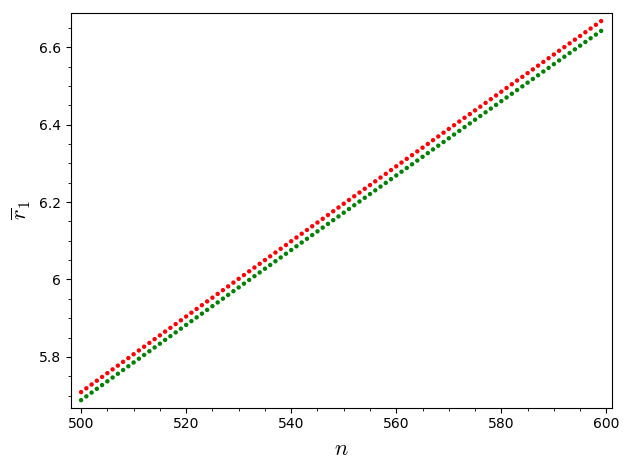
\includegraphics[width=\linewidth]{plot4.png}
  \caption{Comparison of the normalized decoding radius for initial construction(in green) and the generalization(in yellow). Here we took k = 20. }
  \label{fig:gen_int}
\end{figure}


\subsection{Was it all worth it?}
\label{subsec:improvement_integers}


As it turns out factorization of $m$ does not affect the decoding radius substantially. It can only introduce a minor improvement. We prove that with the following lemma:

\begin{lemma}\label{lemma:no_imrovement}
Assume the primes $p_{1}, \dots, p_{n}$ are the same for both lattices. If $a \cdot m \sim b \cdot m' \sim e^n$, when $n \rightarrow \infty$ Then
\[
    \frac{\bar r_{m}^{(1)}}{\bar r_{m'}^{(1)}} \rightarrow 1, n \rightarrow \infty
\]
\end{lemma}
\begin{proof}
    The proof is in the appendix \ref{app:B}
\end{proof}



\section{New Construction for Polynomial Lattices}
\label{sec:polynomials}



\subsection{Definition of Polynomial Lattices}
\label{subsec:def_polynomials}


Let us set parameters a prime power $q$ and integers $k$, $d$ and $n$. Let $\FF_{q}[x]$ be polynomial ring over a field  $\FF_{q}$. We take a set of $k$ irreducible polynomials $c_{j}(x) \in \FF_{q}[x]$, $j =1, ...,k$ of degree $d$. According to the analogue of the prime number theorem for polynomials $k$ must not be greater than $\frac{q^d}{d}$.

Define $c(x) \coloneqq \prod_{j = 1}^{k} c_{j}(x)$. We are going to work in the multiplicative group of the quotient ring of  $\FF_{q}[x]$ with respect to $c(x)$.
Chinese Remainder Theorem helps to determine the structure of $\big(\FF_{q}[x]/c(x)\big)^{*}$:
\[
    \big(\FF_{q}[x]/c(x)\big)^{*} \sim \prod_{i=1}^{k}\big(\FF_{q}[x]/c_{i}(x)\big)^{*} \sim \prod_{i=1}^{k}\FF_{q^{d}}^*
\]
Every component is quotient by an irreducible polynomial, therefore it's a field. Multiplicative group of a field is cyclic, so we can consider discrete logarithms in every component of the product to find a lattice basis.

Consider a vector $\alpha = (\alpha_{1}, ... , \alpha_{n}) \in \FF_{q}^{n}$ where $\alpha_{i}$s are pairwise different. Since polynomials $c_{j}(\cdot)$ are irreducible over $\FF_{q}$ neither of $\alpha_{i}$ can be their root. So for all $\alpha_{i}$ we have: $c(\alpha_{i}) \neq 0$.

Now consider a group morphism:
\[
    \psi : \ZZ^{n} \rightarrow \big(\FF_{q}[x]/c(x)\big)^{*}
\]
\[
    (u_{1}, ..., u_{n}) \mapsto \prod_{i=1}^{n}(x - \alpha_{i})^{u_{i}} \pmod{c(x)}
\]

Similarly to previous constructions the lattice is defined as the kernel of the morphism $\psi$:
\[
    \LL = \ker \psi = \{(u_{1}, ..., u_{n}) \in \ZZ^{n} | \prod_{i=1}^{n}(x - \alpha_{i})^{u_{i}} \equiv 1 \pmod{c(x)}\}
\]
We will be calling $\LL$ the polynomial lattice from now on. Applying CRT gives us an equivalent definition for $\LL$:
\[
    \LL = \ker \psi = \{(u_{1}, ..., u_{n}) \in \ZZ^{n} |  \forall 1 \leq j \leq k: \prod_{i=1}^{n}(x - \alpha_{i})^{u_{i}} \equiv 1 \pmod{c_{j}(x)}\}
\]
Supposing we know $\beta_{j}$ a generator of $\big(\FF_{q}[x]/c_{j}(x)\big)^{*}$ for every $j$ we get another representation by computing discrete logarithms in the multiplicative group of every component:
\[
    \LL = \{(u_{1}, ..., u_{n}) \in \ZZ^{n} | \forall 1 \leq j \leq k: \sum_{i=1}^{n}u_{i}log_{\beta_{j}}(x - \alpha_{i}) \equiv 0 \pmod{q^{d} -1}\}
\]
What might cuase a confusion is that each $\log_{\beta_{j}}$ has a different input domain. For every $j$:  $\log_{\beta_{j}}$ acts from $\big(\FF_{q}[x]/c_{j}(x)\big)^{*}$ into $(\ZZ/(q^{d} - 1)\ZZ)$.


\subsection{Lattice computation for polynomials}
\label{subsec:compute_basis_polynomials}


We obtained a parity check representation of $\LL$.
To calculate a basis of $\LL$ we can follow a simplified version of the algorithm for discrete logarithm lattices. We obtain the dual basis by scaling parity check matrix and concatenating it with $I_{n}$. Then we remove linear dependencies and finally obtain primal basis from the dual. So basis computation algorithm has the following steps:

\begin{enumerate}
    \item \label{step1_p} Obtain the parity check representation of $\LL$.
    \item \label{step2_p} Transform it into the basis of $\LL^{*}$.
    \item \label{step3_p} Recover the primal basis from the dual.
\end{enumerate}

\subsubsection{Parity check representation \ref{step1_p}.}
\label{subsubsec:parity_check_polynomials}
To compute the parity check representation of the polynomial lattice we need to compute
$\forall 1 \leq i,j \leq n :$ $log_{\beta_j}(x - \alpha_i) \pmod{q^{d} -1}$ and form them into a matrix. The order of multiplicative group is $q^{d} - 1$ which is not necessarily a smooth integer so we cannot use Pohlig-Hellman \cite{[PH78]} and Pollard-$\rho$ \cite{[Pol78]} approach to compute them efficiently. We are going to choose $q^{d} = n^{O(1)}$ so group order is overall polynomial in the lattice dimension and use Pollard-$\rho$ \cite{[Pol78]} algorithm to compute discrete logarithms.

\subsubsection{Dual basis \ref{step2_p}.}
\label{subsubsec:dual_gen_set_polynomials}

Lemma \ref{lemma:dual_gen_set} gives us a straightforward way to compute the generating set of the dual from a parity check matrix. To obtain its basis we eliminate linear dependencies by reducing the generating matrix to its Hermite noraml form as in the section \ref{subsubsec:hermite_form}.

\subsubsection{Recovering Primal basis from Dual \ref{step3_p} (Theory).}
\label{subsubsec:primal_from_dual_t_polynomials}

In this section $q$ is and arbitrary integer, not related to the lattices cnstructed before.

Lattices that admit a parity check representation are called $q$-ary lattices. They lie between $\ZZ^{n}_{q}$ and $\ZZ^{n}$: $\ZZ^{n}_{q}  \subset \LL \subset \ZZ^{n}$. For this kind of lattices, it's possible to transform the parity check lattice into its basis efficiently. In the algorithm we will rely on the parity check matrix to have a special shape.
\begin{definition}
A matrix $A \in \mathbb{R}^{n \times m}$ is in the systematic form if it has the following form:
\[
A = \big[ I_{n} | A' \big]
\]
Where $I_{n}$ stands for an identity matrix of dimensions $n \times n$ and $A'$ is an arbitrary matrix of dimensions $n \times (m-n)$
\end{definition}

\begin{lemma}\label{coolfact}
    Suppose $\LL$ is defined by a parity check matrix. $\LL = \{x \in \ZZ^{n}: Hx \equiv 0 \pmod{q}\}$ and $H \in \ZZ_{q}^{k \times n}$ is in the systematic form $H = [I_{k}| D]$. Then rows of $G = [-D^{T}| I_{n-k}]$ are generating vectors of the lattice $\LL$ reduced modulo $q$.
\end{lemma}
\begin{proof}
Let us first prove that every vector generated with the matrix $G$ belongs to the lattice. Let us take an arbitrary vector $x$ and prove that $G^{T} \cdot x$ belongs to $\LL$. So $G$ generates a sublattice of $\LL$. If we prove that their determinants coincide we would prove the lemma.
\[
\forall x: H \cdot G^{T}x = [I_{k}|D] \cdot [-D^{T}| I_{n-k}]^{T}x = (D - D)x = 0 \pmod{x}
\]
If $G$ generates the lattice modulo $q$ then
$
G' = \left[ \begin{array}{c|c} -D^{T} & I_{n-k} \\ \hline qI_k & 0 \end{array}\right]
$
generates all of the lattice $\LL$. $det(G') = q^{k}$. It is left to prove that $\LL$ has the same determinant.
ToDo: finish writing the proof.
\end{proof}

\begin{corrolary}
Suppose the matrix $H$ is in permuted systematic form $e.g. \exists P - \text{ column permutation matrix } P \cdot H = [I | D]$. Then $P \cdot G$ are generating vectors of the lattice $\LL$ reduced modulo $q$.
\end{corrolary}
\subsubsection{Recovering Primal basis from Dual \ref{step3_p} (Practice).}
\label{subsubsec:primal_from_dual_pr_polynomials}

Let us build an algorithm specific to the polynomial lattices. First in our case $q \rightarrow q^{d} -1$. Now $q$ means a prime power - the modulus of the base field $\FF_{q}$.

At the start of this step of lattice computation we are given the parity check matrix if the polynomial lattice. The lattice is the set of solutions to a homogeneous equation modulo $q^{d} -1$ defined by the parity check matrix, therefore, none of the elementary trasformations modulo $q^{d} -1$ can change it. So we can apply Gaussian elimination to reduce it to the systematic form.

Here $q^{d} -1$ is not a prime number, so some of the elements of $H$ might not be invertible modulo $q^{d} -1$, and we cannot render them equal to one. That is why it is useful to have permuted systematic form. We can then try to invert elements of a particular row until we find an invertible one. In practice the algorithm is able to reduce every matrix to its systematic form, so we make an assumption that there's not so many element we cannot invert.

Using Lemma \ref{coolfact} we can obtain the set of generating vectors $G$ of the polynomial lattice $\LL$ modulo $q$. Since we are dealing with the q-ary lattice, to obtain the basis of the $\LL$ itself we need to add the basis of $\ZZ^{n}_{q}$ and remove resulting linear dependencies. It is not strictly nessesary to perfom these steps as having $G$ we can craft points of the lattice $\LL$.

Let us put all the steps together in an algorthm:
\begin{enumerate}
    \item Reduce the parity check matrix to its permuted systematic form.
    \item Transform it into the generating matrix modulo $q$.
    \item Concatenate with $q \cdot I_{n}$.
    \item Reduce obtained matrix to its Hermite normal form.
\end{enumerate}


\subsection{Decoding algorithm modification}
\label{subsec:decoding_polynomials}

We could check now if the framework of the decoding algorithm developped before wil fit this new setting. In this section we discuss the modification we need to make and the decoding radius we can achieve with this approach. Modifying the algorithm to treat polinomials instead of integers leads to the following steps.

\begin{enumerate}
    \item Round every coordinate to $t$ to deal only with discrete error $\lfloor t \rceil = v + \lfloor e \rceil$. Note $e' = \lfloor e \rceil$, $t' = \lfloor t \rceil$.
    \item Compute $\psi(t) = \prod_{i=1}^{n}(x - \alpha_{i})^{v_{i} + e'_i} \pmod{c(x)} = \prod_{i=1}^{n}(x - \alpha_{i})^{e'_i} \pmod{c(x)}$.
    \item \label{step:rfr} Reconstruct the numerator $n$ and the denominator $d$ of $\prod_{i=1}^{n}(x - \alpha_{i})^{e'_i}$ that correspond to positive and negative parts of the error.
    \item Recover prime number factorization of $n$ and $d$ using trial division. Powers of primes will be the coordinates of our error.
    \item Subtract just recovered error from $t'$.
\end{enumerate}

Except for the step \ref{step:rfr} translates directly to the case of polynomials. Step \ref{step:rfr} needs more work, let us discuss rational function reconstruction in more detail.

\subsubsection{Rational function reconstruction \ref{step:rfr}}
\label{subsubsec:rfr}
In the work of \cite{[KM06]} authors study rational function reconstruction in depth.  Given $g,f$ the goal is to find $n, d \in \mathbb{F}[x]$ that $deg(n) + deg(d) < \frac{deg(f)}{2}$ and $\frac{n}{d} = g \pmod{f}$ The main algorithm the discuss is based in Extended Euclidean Algorithm(EEA). We perform extended euclidean division and the select a step where the degree of the xcurrent quotient is greater or equal to $\frac{deg f}{2}$. The authors refer to it as Wang's algorithm. Here is its formal description.

\begin{algorithm}
\caption{RFR}\label{RFR}
\begin{algorithmic}[1]
\Procedure{Reconstruct}{$f,g$}
    \State $r_0 = f$  $r_1 = g$
    \State $t_0 = 0$  $t_1 = 1$
    \State $q = 1$
    \While{$deg(q) \leq \frac{deg(f)}{2}$}
        \State $q = r_0 // r_1$
        \State $(r_0, r_1) = (r_1, r_0 - qr_1)$
        \State $(t_0, t_1) = (t_1, t_0 - qt_1)$
    \EndWhile
    \If{$GCD(r_0, t_0) \neq 1$ or $deg(r_0) + deg(t_0) \geq \frac{deg(f)}{2}$}
        \State \Return FAIL
    \Else:
            \State \Return  $(\frac{r_0}{lc(t_0)}, \frac{t_0}{lc(t_0)})$
    \EndIf
\EndProcedure
\end{algorithmic}
\end{algorithm}
Here function $lc()$ outputs the leading coefficient of the input polynomial.


Correctness of this algorithm follows from the following two lemmas. The first one proves that under certain conditions one of the rows of EEA contains the correct $n$ and $d$. The second lemma tells us how to select the correct row.

\begin{lemma}
Let $\mathbb{F}$ be a field, $f, g, r, s, t \in \mathbb{F}[x]$ with $r = sf + tg$, $t \neq 0$, $deg(f) > 0$, and $deg(r) + deg(t) <deg(f)$.
Suppose $r_i, s_i, t_i$ for $0 \leq i \leq l + 1$ be the elements of the ith iteration in the Extended Euclidean Algorithm(EEA) for $f$ and $g$ (e.i. $r_i = s_if + t_ig$). \\
Then there exists a nonzero element $\alpha \in \mathbb{F}[x]$ such that $r = \alpha r_j$, $s = \alpha s_j$, $t = \alpha t_j$, where $deg(r_j) \leq deg(r) < deg(r_{j-1})$
\end{lemma}
\begin{proof}
Find the proof in \cite{[GG13]} (Lemma 5.15 page 116)
\end{proof}

So if the solution exists it must be one of the pairs $(r_i, t_i)$ of the EEA.

\begin{lemma}
Let $\mathbb{F}$ be a field $f,g,n,d \in \mathbb{F}[x]$ are polynomials such that $lc(d) = 1$, $gcd(n,d) = gcd(f,d) = 1$ and $g = frac{n}{d} \pmod{f}$. Let $j$ be the index of a quotient with maximal degree in the EEA for $f$ and $g$. If $deg(f) > 2(deg(n) + deg(d))$ the $j$ is unique and $n = r_j$, $d = t_j$
\end{lemma}
\begin{proof}
Find the proof in \cite{[KM06]} (Lemma 2.3 page 186)
\end{proof}


\subsubsection{Factorization by trial division}
\label{subsubsec:factoring_polynomials}
Input: A polynomial $g$ such that $deg(g) \leq m$ whose roots are among $\alpha_1, \dots , \alpha_n \in \mathbb{F}_q$\\
Output: $e_1, \dots , e_n$ s.t. $g = \prod_{i = 1}^{n}(x - \alpha_i)^{e_i}$\\
There's only $n$ possible roots, one trial division takes $O(m)$ time and the number of factors is bounded by $m$. So overall complexity is $O(m^2n)$.


\subsection{Decoding radius}
\label{subsec:radius_polynomials}

Rational function reconstruction puts an upperbound on how much error this algorithm can decode. Let us first consider a simpler case where every coordinate of the error in positive, so the step \ref{step:rfr} becomes trivial. The goal of this section is to find the parameters which provide maximal normalized decoding radius for arbitrary discrete error and calculate the this upperbound.

\subsubsection{Only positive discrete error}
\label{subsubsec:positive_error}
Suppose we receive $t = u + e$ where $u \in \mathcal{L}$, $\|e\|_1 \leq r_1$ and $\forall i: e_i \in \mathbb{N}$. Then we can compute
\[
\prod_{i = 1}^{n}(x - \alpha_i)^{t_i} = \prod_{i = 1}^{n}(x - \alpha_i)^{u_i}\prod_{i = 1}^{n}(x - \alpha_i)^{e_i} \pmod{c(x)}
\]
If $\|e\|_1 = \sum_{i =1}^{n} e_i \leq deg(c) = d \cdot k$ the operation above will give us exactly the polynomial $\prod_{i = 1}^{n}(x - \alpha_i)^{e_i}$. Then we can recover $e_i$, $1 \leq i \leq n$ from the factorization.\\
So $l_1(r_1) = d \cdot k$.

Due to the nature of the bound above it is natural to talk about the length $r_1$ in $l_1$ norm.


\subsubsection{Arbitrary discrete error}
\label{subsubsec:discrete_error}
Now we have $\forall i: e_i \in \mathbb{Z}$. Then
\[
\prod_{i = 1}^{n}(x - \alpha_i)^{t_i} \pmod{c(x)} = \prod_{i = 1}^{n}(x - \alpha_i)^{e_i} = \frac{\prod_{i \in I}(x - \alpha_i)^{e_i}}{\prod_{j \in J}(x - \alpha_j)^{-e_j}}
\]

\begin{lemma}
Given $g,c$ where $deg(c) = d \cdot k$ we can recover $f_{1}, f_{2} \in \mathbb{F}[x]$ that  $\forall i = 1;2$: $deg(f_{i}) \leq \floor{\frac{dk}{2}}$ and $\frac{f_{1}}{f_{2}} = g \pmod{c}$ in polynomial time.
\end{lemma}

So we can decode every message for which $\|e\|_1 = \sum_{i =1}^{n} |e_i| \leq \floor{\frac{dk}{2}}$

If we know more about the shape of the error the upper bound becomes even better. We can reconstruct $g = \frac{n}{d} \pmod{f}$ if it is known that $deg n < N$, $deg d < D$ where $N + D < deg f$ refer to \cite{[KM06]} for more information.


\subsubsection{Normalized radius}
\label{subsubsec:normalized_discrete_error}
From the bound on the error we already have we obtain the mormalized raduis $\bar{r}_1 = \frac{dk}{2 \cdot det(\mathcal{L})^{1/n}}$ where $det(\mathcal{L}) = \Phi(c(x)) = (q^{d} - 1)^{k}$.
\[
\bar{r}_1 = \frac{dk}{2 \cdot (q^{d} - 1)^{k/n}}
\]
Let us optimize the values of $d$ and $k$.

We have the following constraints:
\begin{enumerate}\label{constraints}
    \item $q^d = n^{O(1)}$
    \item $dk < q^{d}$
    \item $n \leq q$
\end{enumerate}
From these we can immediately conclude that $d$ must be constant. \\

To obtain not more than a logarithmic gap from Minkowski's bound we need the following asymptotics: $q = a \cdot n$, $d = b$, $k =  c \cdot \frac{n}{\log(n)}$. What we are going to do next is finding optimal values for parameters $a, b$ and $c$. We want to maximize the following function:
\[
\bar{r}_1 = \frac{bc \cdot n}{2\log(n)((an)^{b} - 1)^{c/\log(n)}}  \sim \frac{bc \cdot n}{2e^{bc}\log(n)}
\]
 Parameter $a$ by constraint 3 in \ref{constraints} should be greater or equal to 1.
 \[
    \frac{bc \cdot n}{2\log(n)((an)^{b} - 1)^{c/\log(n)}} \leq \frac{bc \cdot n}{2\log(n)(n^{b} - 1)^{c/\log(n)}}
 \]

The choice of $a$ is independent from choices of $b$ and $c$ so we can configure it to the smalles possible value $a = 1$.

The function we are considering with fixed parameters $c, b$ tend to the same value as $\frac{bc \cdot n}{2\log(n)n^{cb/\log(n)}}$. To simplify the analysis we will find the best parameters for the latter.

Note $d \coloneqq bc$, $f_n(d) = \frac{d \cdot n^{1 - \frac{d}
{\log(n)} }}{2\log(n)}$.
We would like to prove that for any value of $n$, $argmax(f_n(d)) = 1$
\[
\begin{split}
    f_n'(d) & = \frac{n^{1 - \frac{d}
    {\log(n)}}}{2\log(n)} + \frac{d \cdot n^{1 - \frac{d}
    {\log(n)}} \cdot \log(n) \big(-\frac{1}{\log(n)}\big)}{2\log(n)} \\
    & = \frac{n^{1 - \frac{d}{\log(n)}}}{2\log(n)}(1-d)
\end{split}
\]
$d = 1$ is the only solution to the equation $f_n'(d) = 0$. It is easy to verify that it corresponds to the maximum of $f_n(d)$ and it doesn't depend on the value of $n$.

Therefore, $b \cdot c = 1$. In practice we fix $b = 2, c = \frac{1}{2}$. In the end, the decoding radius our algorithm achieves is
\[
    \bar{r}_1 = \frac{n}{2 \cdot \log(n)(n^{2} - 1)^{1/2\log(n)}}
\]

\subsection{Comparing the decoding radius of the algorithms}
\label{sec:comparison}

For the first family final normalized error radius that the algorithm can handle is:
\[
    \bar{r}_1 = \frac{\ln(m/2)}{4 \cdot \varphi(m)^{1/n} \cdot \ln((n+1)\ln(n+1))}
\]
And for the second construction it is much better:
\[
    \bar{r}_1 = \frac{n}{2 \cdot \log(n)(n^{2} - 1)^{1/2\log(n)}}
\]
But both of them are still logatihmically far from Minkowski's bound. The figure \ref{fig:everything} will help you to see the difference in practice.

\begin{figure}
  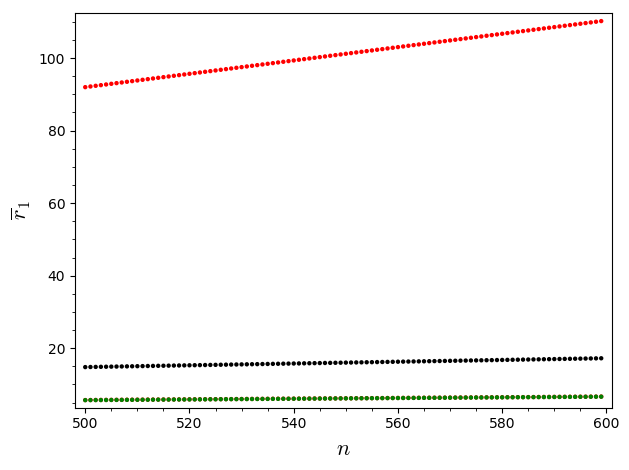
\includegraphics[width=\linewidth]{plot5.png}
  \caption{Comparison of all algorithms and theoretical upperbound(in red): basic algorithm for integer lattice(in green), algorithm for polynomial lattices(in blue)}
  \label{fig:everything}
\end{figure}

\section{LLXY17 Cryptanalysis}
\label{sec:cryptanalysis}

Let us give a high level description of the encryption scheme presented in \cite{[LLXY17]}. It is based on the family of polynomial lattices that we described above. The public key of Alice is a matrix $G$ that enerates a sublattice of a polynomial lattice $\LL$. When Bob wants to send a message $m$ to Alice he generates a random noise $ e \in \{0,1\}^{n}$ of hamming weight $w$ and sends the ciphertext $c = Gm + e$.

Alice's private key containes parameters $c(x)$ and $(\alpha_1, \dots, \alpha_n)$ used to construct the lattice $\LL$. To decode the message Alice performs error decoding algorithm discussed in the section \ref{subsec:decoding_polynomials}. As we saw, for the decoding procedure to work $w$(the $l_1$ norm of $e$) should be less than the upperbound on the error.

We given the ciphertext $c$ we would like to obtain the message without the key. Having the generating matrx $G$ we can obtain the parity check representation $H$ of $\LL$. Multiplying the ciphertext by $H$ we obtain:
\[
    H \cdot c = H \cdot Gm + H \cdot e = H \cdot e
\]

We would like to try evey possible value of the error until $H \cdot c = H \cdot e$. If we can learn the value of the error, we can subtract it from the cipher text and obtain the message multiplying by $G^{-1}$.

Let us consider three different approaches to make the bruteforce attack more efficient.

We compute the cost of every attack in the appendix \ref{app:A}


\subsection{Information Set Decoding Attack}

We take a vector $y \in \ZZ_q^{k}$, a matrix $A \in \ZZ_q^{k \times n}$. It can be reduced to its permuted systematic form $H  = U \cdot A = [I_{k}|D]$.


The goal is to find a vector $x \in \{0,1\}^{n}$ with small Hamming weight $|x| = w$ that
\[
Ax = y
\]

Or equivalently $Hx = U\cdot Ax = Uy =: t$, here we can use our knowledge about the shape of $H$.

In this attack we partition $x$ on two vectors $x_1 \in \{0,1\}^{k}$ and  $x_2  \in \{0,1\}^{n-k}$ so we have
\[
t = x_1 + D \cdot x_2
\]
We make a bet of the weight partition between $|x_1| = w_1$ and $|x_2| = w_2$, where $w_1 + w_2 = w$. Now we enumerate only the possible values of $x_2$, compute $x_1 = t - D \cdot x_2$ and check if it satisfies $|x_1| = w_1$. If we don't find a correct pair with this weight distribution, we rerandomize H and t and start over. Here we present the pseudoce of the attack. \ref{ISD}
\begin{algorithm}
\caption{ISD attack}\label{ISD}
\begin{algorithmic}[1]
\Procedure{Decoding}{$A,y$}
    \State Reduce A it's randomized systematic form: $(I_k |D)$
    \For{$x_2$ of weight $w_2$}
        \State compute $x_1 = t - Dx_2$
        \If {$|x_1| = w_1$ and contains only $0,1$}
        \State \Return Derandomize $x = (x_1, x_2)$
        \EndIf
    \EndFor
\State \textbf{goto} \emph{line 2}.
\EndProcedure
\end{algorithmic}
\end{algorithm}

\subsection{Meet in the Middle}
In this attack we have the same goal but no information about the form of the matrix A.
We partition $x$ and $A$ on two equal parts: $A = [A_1 | A_2]$, $x = (x_1 | x_2)$.
Then $Ax = y$ is equivalent to
\[
    A_1x_1 + A_2x_2 = y
\]
If we can find vectors $x_1$ and $x_2$ for which values $A_1x_1$ and $y - A_2x_2$ coincide. Here we make a bet that weight is distributed equall between the two parts.Similarly we present the pseudocode of the attack below \ref{MitM}.


\begin{algorithm}
\caption{MitM attack}\label{MitM}
\begin{algorithmic}[1]
\Procedure{Decoding}{$A,y$}
    \State Generate random matrix $U$
    \State $(A_1|A_2) \gets A \cdot U$
    \State $t = y \cdot U$
    \For{$x_1$ of weight $\frac{w}{2}$}
    \State compute $A_1x_1$
    \State store in the hash table
    \EndFor
    \For{$x_2$ of weight $\frac{w}{2}$}
    \State compute $t - A_2x_2$
    \State look up in the hash table for a collision
    \If {collision found}
        \State \Return $x = (x_1, x_2)$
    \EndIf
    \EndFor
\State \textbf{goto} \emph{line 2}.
\EndProcedure
\end{algorithmic}
\end{algorithm}

\subsection{Combining the two approaches.}

Now we would like to combine Information Set Decoding attack with Meet in the Middle approach to make it even more efficient.

We return to the case when $A$ is reduced to the systematic form $H = U \cdot A = [I_{k}| D_1 | D_2]$ we partition $x = (x_0 |x_1 |x_2)$ on three vectors $x_0 = \in \{0,1\}^{k}$, $x_1,x_2 \in \{0,1\}^{\frac{n-k}{2}}$. Then
\[
  Ax = x_0 + D_1x_1 + D_2x_2
\]

We make bet that $|x_0| = w_1$, $|x_1| = |x_2| = \frac{w_2}{2}$ and perform Meet-in-the-Middle attack. Now we would like to find \textbf{approximate} collisions between $D_1x_1$ and all possible $t - D_2x_2$

For that we desing a compression function $f$ that will often map close vectors to the same value. It operates as follows:
\[
\forall v = (v_1, \dots , v_k)\in \ZZ_{q}^{k}: f_{p}(v) = (\lfloor v1/p \rceil, \lfloor v2/p \rceil, \dots, \lfloor vk/p \rceil)
\]
Here $p$ is a parameter of the function.

We store a table of $f(D_1x_1)$ in memory and look-up there for $t - D_2x_2$. We will need to deal with false positives and false negatives in this collision search. Too many false positives can increase the cost of the search for every randomization of the public key matrix and too many false negatives can increase the number of randomizations themselves. To ease the analysis we present pseudocode of the algorithm. \ref{algo}


\begin{algorithm}
\caption{ISD+MitM attack}\label{algo}
\begin{algorithmic}[1]
\Procedure{Decoding}{$A,y$}
    \State Reduce A it's randomized systematic form: $(I_k |D_1|D_2)$
    \For{$x_1$ of weight $\frac{w_2}{2}$}
    \State compute $f_{p}(D_1x_1)$
    \State store in the hash table
    \EndFor
    \For{$x_2$ of weight $\frac{w_2}{2}$}
    \State compute $f_{p}(t - D_2x_2)$
    \State look up in the hash table for a collision
    \If {collision found}
        \State compute $D_1x_1$
        \State compute $x_0 = t - D_2x_2 - D_1x_1$
        \If {$|x_0| = w_1$ and contains only $0,1$}
        \State \Return Derandomize $x = (x_0, x_1, x_2)$
        \EndIf
    \EndIf
    \EndFor
\State \textbf{goto} \emph{line 2}.
\EndProcedure
\end{algorithmic}
\end{algorithm}

\subsection{Adding negative errors}
\label{subsec:negative_error_improvement}
Our algorithm allows to decode errors of both signs efficiently, so adding it will improve security of [LLXY17] encyption scheme. Let us estimate how resistant is the scheme agains our most efficient attack when it uses $ e \in \{0,1\}^{n}$ and $ e \in \{0,1,-1\}^{n}$ of the same $l_1$ norm. The costs and imprevement are presented in the following table.\\

\begin{tabular}{ |l||p{2,5cm}|p{2,5cm}|p{2,5cm}|p{2,5cm}|p{2cm}|  }
 \hline
 \multicolumn{6}{|c|}{Cost of attacks for different parameters} \\
 \hline
 Parameters & Bruteforce & ISD & MitM & IDS+MitM & imrovement rate \\
 \hline
 \makecell{n = 100.0 \\ k = 10.0 \\ w = 5.0 \\ q = 100.0} & 4.517251e+09 & 2.960902e+07 & 2.116580e+05 & 2.366108e+05 & \\
 \hline
 Ternary & 1.445520e+11 & 6.725278e+07 & 1.197318e+06 & 3.293097e+05 & 2\\
 \hline
 \makecell{ n = 100.0 \\ k = 10.0 \\ w = 9.0 \\ q = 100.0} & 1.902232e+14 & 2.801449e+11 & 8.084476e+07 & 2.006729e+07 &  \\
 \hline
 Ternary & 9.739427e+16 & 1.699224e+12 & 1.829308e+09 & 1.854533e+08 & $2^{3}$ \\
 \hline
 \makecell{n = 500.0 \\ k = 40.0 \\ w = 30.0 \\ q = 500.0} & 1.792122e+51 &  3.963162e+39 & 3.737340e+27 & 2.087190e+24 &  \\
 \hline
 Ternary & 1.924276e+60 & 1.091922e+41 & 1.224651e+32 & 3.433996e+27 & $2^{11}$\\
 \hline
 \makecell{n = 1000.0 \\ k = 72.0 \\ w = 50.0 \\ q = 1000.0} & 3.473881e+88 & 2.056657e+67 & 3.262500e+46 &  1.362168e+41 &  \\
 \hline
 Ternary & 3.911243e+103 & 8.987320e+68 & 1.094713e+54 & 3.432411e+46 & $2^{18}$ \\
 \hline
\end{tabular}

\subsection{LLXY17 parameter selection}
\label{subsec:param_improvement}

We would also like to comment on parameter selection made for the scheme. In the following table we present costs of the attack for the smallest and largest parameters suggested by \cite{[LLXY17]} for their encryption scheme. Their estimate seccurity level for the first one is $2^{106}$ and $2^{119}$. With our best attack we are able to break it with average cost of $2^{25}$ and $2^{26}$ which is feasible in practice. \\


\begin{tabular}{ |l||p{2,5cm}|p{2,5cm}|p{2,5cm}| }
 \hline
 \multicolumn{4}{|c|}{Cost of attacks for LLXY17 parameters } \\
 \hline
 Parameters & Claimed security & IDS+MitM cost & in binary \\
 \hline
 \makecell{n = 230.0 \\ k = 201.0 \\ w = 28.0 \\ q = 263.0} & $2^{106}$ & 2.778036e+07 & $2^{25}$ \\
 \hline
 \makecell{n = 260.0 \\ k = 228.0 \\ w = 31.0 \\ q = 293.0} & $2^{119}$ & 4.523610e+07 & $2^{26}$ \\
 \hline
\end{tabular}
\\

In concusion parameters taken for this scheme need to be seriously reconsidered.

\section{Future work}

The main question left to answer is what are the correct parameters to use in the scheme of \cite{[LLXY17]}. For that we need to take into account the cost of our most efficient attack, the attacks discussed in the original paper and the constraints of our decoding algorithm. After the parameter are computed we need to see if the scheme is still practical.


\appendix
\section{Proof of Lemma \ref{lemma:no_imrovement}}
\label{app:B}
\begin{proof}
Since the primes are the same, they are also bounded by the same constant $B$ so the term $\frac{1}{4 \ln(B)}$ cancels out in the numerator and denominator.
\[
\begin{split}
\frac{\bar r_{m}^{(1)}}{\bar r_{m'}^{(1)}}
& = \frac{\ln(m/2) \cdot \varphi(m')^{1/n}}{\ln(m'/2) \cdot \varphi(m)^{1/n}} \\
& = \frac{\ln(e^n/2a) \cdot \varphi(m')^{1/n}}{\ln(e^n/2b) \cdot \varphi(m)^{1/n}} \\
& = \frac{\varphi(m')^{1/n}}{\varphi(m)^{1/n}}
\end{split}
\]
We apply a few classic results to estimate the growth of $\varphi(n)$ \cite{[HW09]}:
\[
    \limsup\limits_{n \rightarrow \infty} \frac{\varphi(n)}{n} = 1
\]
\[
    \liminf\limits_{n \rightarrow \infty} \frac{\varphi(n) \cdot \ln\ln(n)}{n} = e^{-\gamma}
\]
where $\gamma$ is the Euler constant, $e^{-\gamma} = 0.56145948\dots$
\[
\begin{split}
\lim_{n \rightarrow \infty} \frac{\varphi(m')^{1/n}}{\varphi(m)^{1/n}}
& \leq \frac{\limsup\limits_{n \rightarrow \infty} \varphi(m')^{1/n}}{\liminf\limits_{n \rightarrow\infty}\varphi(m)^{1/n}} \\
& = \lim_{n \rightarrow \infty} \bigg(\frac{m \cdot \ln\ln (m')}{m'}\bigg)^{1/n} \\
& = \lim_{n \rightarrow \infty} (\ln\ln(e^n/b))^{1/n} = 1
\end{split}
\]
\end{proof}
\section{Calculating the cost of attacks}
\label{app:A}

\subsection{ISD: Binary case}
The average cost of such algorithm can be calculated as
\[
T = \frac{x_2\text{ bruteforce cost}}{Pr(w_2\text{ is a correct bet on the weight of }x_2)}
\]
Let us compute the values above.
The numerator:
\begin{itemize}
    \item Step 3-4: $O(k\cdot n^2)$
    \item Step 5: $O(k \cdot (n-1) \cdot (k-1))$
    \item Step 6-11: $O(k \cdot w_2 \cdot \binom{n-k}{w_2})$
\end{itemize}
In total we have: $k \cdot (n^2 + (n-1)(k-1) + w_2\binom{n-k}{w_2})$
The denominator:
\[
\begin{split}
    Pr(w_2\text{ is a correct bet on the weight of }x_2) & = Pr(|x_2| = w_2||x| = w) \\
    & = \frac{\binom{n-k}{w_2} \cdot \binom{k}{w_1}}{\binom{n}{w}}
\end{split}
\]
Therefore
\[
T = \frac{k\cdot\binom{n}{w}\cdot(n^2 + (n-1)(k-1) + w_2\binom{n}{w_2})}{\binom{k}{w_1}\binom{n-k}{w_2}}
\]
\subsection{ISD: Ternary case}
The numerator:
Only the number of choices for $x_2$ change
\[
    k\cdot(n^2 + (n-1)(k-1) + w_2\binom{n-k}{w_2}\cdot2^{w_2})
\]
The denominator:
\[
\begin{split}
    Pr(w_2\text{ is a correct bet on the weight of }x_2) & = Pr(|x_2| = w_2||x| = w) \\
    & = \frac{\binom{n-k}{w_2} \cdot \binom{k}{w_1}}{\binom{n}{w}}
\end{split}
\]
Therefore
\[
T = \frac{k\cdot\binom{n}{w}\cdot(n^2 + (n-1)(k-1) + w_2\binom{n}{w_2}\cdot2^{w_2})}{\binom{k}{w_1}\binom{n-k}{w_2}}
\]

To minimize the average cost we take an optimal value of $w_1$ calculated with a script.

\subsection{MitM: Binary case}


Here we bet the weight is distributed equaly on both sides. So the average cost can be calculated as follows:
\[
  T = \frac{\text{cost of finding a collision}}{Pr(|x_1| = |x_2| = w/2| |x| =w)}
\]
Numerator:
\begin{itemize}
    \item Step 2: $n*k*log(q)$
    \item Step 3-4: $O(k \cdot n^2)$
    \item Step 5-8: $O(k \cdot \frac{w}{2} \cdot \binom{n/2}{w/2})$
    \item Step 9-15: $O(k \cdot \frac{w}{2} \cdot \binom{n/2}{w/2})$
\end{itemize}

In total:

TIME COST = $O(k \cdot (n^2 + w\binom{n/2}{w/2}))$

We need to store every $x_1$


MEMORY COST = $\binom{n/2}{w/2} \cdot log(n) \cdot \frac{w}{2}$

Denominator:
$Pr(|x_1| = |x_2| = w/2) = \frac{\binom{n/2}{w/2}^{2}}{\binom{n}{w}}$

Total cost(only time):
\[
  T = \frac{k \cdot \binom{n}{w} \cdot (n^2 + w\binom{n/2}{w/2})}{\binom{n/2}{w/2}^2}
\]

\subsection{MitM: Ternary case}

Numerator:

TIME COST = $k \cdot (n^2 + w \cdot \binom{n/2}{w/2} \cdot 2^{w/2})$

We need to store every $x_1$

MEMORY COST = $\binom{n/2}{w/2} \cdot 2^{w/2} \cdot log(n) \cdot \frac{w}{2}$

Denominator:
$Pr(|x_1| = |x_2| = w/2) = \frac{\binom{n/2}{w/2}^{2}}{\binom{n}{w}}$

Total cost(only time):
\[
  T = \frac{k \cdot \binom{n}{w} \cdot 2^{w/2} \cdot (n^2 + w\binom{n/2}{w/2})}{\binom{n/2}{w/2}^2}
\]

\subsection{ISD+MitM: Binary case}


Computational cost:
Let us first compute the cost of running the algorithm when we were lucky to generate such matrix $U$ that we end up finding vector $x$ that satisfies all the coditions.
\begin{itemize}
    \item Step 3-4: $O(k \cdot n^2)$
    \item Step 5: $O(k \cdot (n-1) \cdot (k-1))$
    \item Step 6-9: $O(k \cdot \frac{w_2}{2} \cdot \binom{(n-k)/2}{w_2/2})$
    \item Step 10-19: $O(k \cdot \frac{w_2}{2} \cdot \binom{(n-k)/2}{w_2/2} + k \cdot \{\text{\# positives}\})$
\end{itemize}
In total we have: $k \cdot (n^2 + (n-1)(k-1) + w_2\binom{(n-k)/2}{w_2/2} + + E(\{\text{\# positives}\}))$

Memory cost:
We only store in memory the hash table of $x_1$ in a cell with index $f_{p}(D_1x_1)$ for every $x_1$.
The weight of $x_1$ is small so we only remember the set of nonzero coordinates $log(n) \cdot \frac{w_2}{2}$ Number of such $x_1$: $\binom{(n-k)/2}{w_2/2}$

So the overall complexity is  $\binom{(n-k)/2}{w_2/2} \cdot log(n) \cdot \frac{w_2}{2}$

Total average cost:
\[
    T = \frac{k \cdot (n^2 + (n-1)(k-1) + w_2\binom{(n-k)/2}{w_2/2} + E(\{\text{\# positives}\}))}{Pr(\text{weight distribution bet was successful, there was no false negative in the collision search})}
\]
Let us calculate missing parts of the formula:
\[
\begin{split}
    E(\{\text{\#positives}\}) = \binom{n}{w_2} \cdot Pr(\text{positive})
\end{split}
\]
\[
\begin{split}
    Pr(\text{positive}) & = Pr(\text{collision happens}) \\
    & = \frac{1}{\lfloor q/p \rceil}^{n}
\end{split}
\]

To simplify the notations for the computation of false negatives $y_1 \coloneqq D_1x_1$, $y_2 \coloneqq t-D_2x_2$ let us call $T$ the hash table of $y_1$s. The number of boxes($\lfloor q/p \rceil$) we denote with $b$. We assume that $y_1, y_2$ are distributed uniformly over $\ZZ_q^{k}$ because otherwise we would be able to obtain some information on $x_1$ and $x_2$ and speed up the bruteforce which would break our security assumption(THINK AGAIN ABOUT THIS). $t_i$ signify non-zero coordinates of$x_0$
\[
\begin{split}
    Pr_{y_2}(\text{false negative}) & = Pr_{y_2}(\exists y_1 \in t: f_p(y_1) \neq f_p(y_2), |x_0| \coloneqq |y_2 - y_1| = w_1, x_0 \in \{0,1\}^{k}) \\
    & = Pr_{y_2}(\exists x_0 s.t. |x_0| = w_1, x_0 \in\{0,1\}^{k}: f_p(y_2 - x_0) \neq f_p(y_2), y_2 - x_0 \in T) \\
    & \leq (\text{union bound}) \leq \sum_{x_0} Pr_{y_2}(f_p(y_2 - x_0) \neq f_p(y_2), y_2 - x_0 \in T) \\
    & \leq (\text{union bound}) \leq \sum_{x_0} \sum_{i = 1}^{w_1} Pr_{y_2}((y_2)_{t_i} \in \{kp+1 p=0, \dots b\}, y_2 - x_0 \in T) \\
    & = \sum_{x_0} \sum_{i = 1}^{w_1} \frac{\binom{n-k/2}{w_2/2} \cdot \frac{b}{q}}{q^k} \\
    & = \sum_{x_0} w_1 \cdot \frac{\binom{n-k/2}{w_2/2} \cdot \frac{b}{q}}{q^k} \\
    & = \binom{k}{w_1} \cdot w_1 \cdot \frac{\binom{n-k/2}{w_2/2} \cdot \frac{b}{q}}{q^k}
\end{split}
\]
\[
\begin{split}
    Pr(\text{weight distribution is correct}) & = Pr(|x_0| = w_1, |x_1| = |x_2| = \frac{w_2}{2}) \\
    & = \frac{\binom{n-k/2}{w_2/2}^{2}\binom{k}{w_1}}{\binom{n}{w}}
\end{split}
\]
Putting everything together we obtain the total average cost.

\subsection{ISD+MitM: Ternary case}

Computational cost:
\begin{itemize}
    \item Step 3-4: $O(k \cdot n^2)$
    \item Step 5: $O(k \cdot (n-1) \cdot (k-1))$
    \item Step 6-9: $O(k \cdot \frac{w_2}{2} \cdot \binom{(n-k)/2}{w_2/2} \cdot 2^{w_2/2})$
    \item Step 10-19: $O(k \cdot \frac{w_2}{2} \cdot \binom{(n-k)/2}{w_2/2} \cdot 2^{w_2/2} + k \cdot \{\text{\# positives}\})$
\end{itemize}
In total we have: $k \cdot (n^2 + (n-1)(k-1) + w_2\binom{(n-k)/2}{w_2/2} \cdot 2^{w_2/2} + E(\{\text{\# positives}\}))$

Memory cost:
We only store in memory the hash table of $x_1$ in a cell with index $f_{p}(D_1x_1)$ for every $x_1$.
The weight of $x_1$ is small so we only remember the set of nonzero coordinates $log(n) \cdot \frac{w_2}{2}$ Number of such $x_1$: $\binom{(n-k)/2}{w_2/2} \cdot 2^{w_2/2}$

So the overall complexity is  $\binom{(n-k)/2}{w_2/2} \cdot 2^{w_2/2} \cdot log(n) \cdot \frac{w_2}{2}$

Total average cost:
\[
    T = \frac{k \cdot (n^2 + (n-1)(k-1) + w_2\binom{(n-k)/2}{w_2/2} \cdot 2^{w_2/2} + E(\{\text{\# positives}\}))}{Pr(\text{weight distribution bet was successful, there was no false negative})}
\]
Let us calculate missing parts of the formula:
\[
\begin{split}
    E(\{\text{\# positives}\}) = \binom{n}{w_2} \cdot 2^{w_2/2} \cdot Pr(\text{positive})
\end{split}
\]
\[
\begin{split}
    Pr(\text{positive}) & = Pr(\text{collision happens}) \\
    & = \frac{1}{\lfloor q/p \rceil}^{n}
\end{split}
\]
\[
\begin{split}
    Pr_{y_2}(\text{false negative}) & = Pr_{y_2}(\exists y_1 \in t: f_p(y_1) \neq f_p(y_2), |x_0| \coloneqq |y_2 - y_1| = w_1, x_0 \in \{0,1\}^{k}) \\
    & = Pr_{y_2}(\exists x_0 s.t. |x_0| = w_1, x_0 \in\{0,1\}^{k}: f_p(y_2 - x_0) \neq f_p(y_2), y_2 - x_0 \in T) \\
    & \leq (\text{union bound}) \leq \sum_{x_0} Pr_{y_2}(f_p(y_2 - x_0) \neq f_p(y_2), y_2 - x_0 \in T) \\
    & \leq (\text{union bound}) \leq \sum_{x_0} \sum_{i = 1}^{w_1} \mathds{1}_{(x_0 = 1)}Pr_{y_2}((y_2)_{t_i} \in \{kp+1 p=0, \dots b\}, y_2 - x_0 \in T) \\
    & + \mathds{1}_{(x_0 = -1)}Pr_{y_2}((y_2)_{t_i} \in \{kp-1 p=0, \dots b\}, y_2 - x_0 \in T) \\
    & = \sum_{x_0} \sum_{i = 1}^{w_1} \frac{\binom{n-k/2}{w_2/2} \cdot \frac{b}{q}}{q^k} \\
    & = \sum_{x_0} w_1 \cdot \frac{\binom{n-k/2}{w_2/2} \cdot \frac{b}{q}}{q^k} \\
    & = \binom{k}{w_1} \cdot 2^{w_1} \cdot w_1 \cdot \frac{\binom{n-k/2}{w_2/2} \cdot \frac{b}{q}}{q^k}
\end{split}
\]

\[
\begin{split}
    Pr(\text{weight distribution is correct}) & = Pr(|x_0| = w_1, |x_1| = |x_2| = \frac{w_2}{2}) \\
    & = \frac{\binom{n-k/2}{w_2/2}^{2}\binom{k}{w_1}}{\binom{n}{w}}
\end{split}
\]
Putting everything together we obtain the total average cost.

\bibliography{report}
\bibliographystyle{ieeetr}

\end{document}
